%% BioMed_Central_Tex_Template_v1.06
%%                   %
% bmc_article.tex      ver: 1.06 %
%                    %

%%IMPORTANT: do not delete the first line of this template
%%It must be present to~enable the BMC Submission system to~
%%recognise this template!!

%%%%%%%%%%%%%%%%%%%%%%%%%%%%%%%%%%%%%%%%%
%%                   %%
%% LaTeX template for BioMed Central %%
%%   journal article submissions   %%
%%                   %%
%%     <14 August 2007>      %%
%%                   %%
%%                   %%
%% Uses:                %%
%% cite.sty, url.sty, bmc_article.cls %%
%% ifthen.sty. multicol.sty		  %%
%%				   	  %%
%%                   %%
%%%%%%%%%%%%%%%%%%%%%%%%%%%%%%%%%%%%%%%%%


%%%%%%%%%%%%%%%%%%%%%%%%%%%%%%%%%%%%%%%%%%%%%%%%%%%%%%%%%%%%%%%%%%%%%
%%                                 %%	
%% For instructions on how to~fill out this Tex template      %%
%% document please refer to~Readme.pdf and the instructions for  %%
%% authors page on the biomed central website           %%
%% http://www.biomedcentral.com/info/authors/           %%
%%                                 %%
%% Please do not use \input{...} to~include other tex files.    %%
%% Submit your LaTeX manuscript as one .tex document.       %%
%%                                 %%
%% All additional figures and files should be attached       %%
%% separately and not embedded in the \TeX\ document its~elf.    %%
%%                                 %%
%% BioMed Central currently use the MikTex distribution of     %%
%% TeX for Windows) of TeX and LaTeX. This is available from   %%
%% http://www.miktex.org                      %%
%%                                 %%
%%%%%%%%%%%%%%%%%%%%%%%%%%%%%%%%%%%%%%%%%%%%%%%%%%%%%%%%%%%%%%%%%%%%%


\NeedsTeXFormat{LaTeX2e}[1995/12/01]
\documentclass[10pt]{bmc_article}  



% Load packages
\usepackage{cite} % Make references as [1-4], not [1,2,3,4]
\usepackage{url} % Formatting web addresses 
\usepackage{ifthen} % Conditional 
\usepackage{multicol}  %Columns
\usepackage[utf8]{inputenc} %unicode support
\usepackage{graphicx}
\usepackage{mathtools}
%\usepackage[applemac]{inputenc} %applemac support if unicode package fails
%\usepackage[latin1]{inputenc} %UNIX support if unicode package fails
\usepackage{color,soul}
\usepackage{amsmath, amssymb}
\usepackage{algorithm2e}
\urlstyle{rm}


\newcommand{\nc}[1]{\begin{flushleft}\hl{[#1]}\end{flushleft}}

 
 
%%%%%%%%%%%%%%%%%%%%%%%%%%%%%%%%%%%%%%%%%%%%%%%%%	
%%                       %%
%% If you wish to~display your graphics for  %%
%% your own use using includegraphic or    %%
%% includegraphics, then comment out the   %%
%% following two lines of code.        %%  
%% NB: These line *must* be included when   %%
%% submitting to~BMC.             %% 
%% All figure files must be submitted as   %%
%% separate graphics through the BMC     %%
%% submission process, not included in the  %% 
%% submitted article.             %% 
%%                       %%
%%%%%%%%%%%%%%%%%%%%%%%%%%%%%%%%%%%%%%%%%%%%%%%%%           


%\def\includegraphic{}
%\def\includegraphics{}



\setlength{\topmargin}{0.0cm}
\setlength{\textheight}{21.5cm}
\setlength{\oddsidemargin}{0cm} 
\setlength{\textwidth}{16.5cm}
\setlength{\columnsep}{0.6cm}

\newboolean{publ}

%%%%%%%%%%%%%%%%%%%%%%%%%%%%%%%%%%%%%%%%%%%%%%%%%%
%%                       %%
%% You may change the following style settings %%
%% Should you wish to~format your article    %%
%% in a~publication style for printing out and %%
%% sharing with colleagues, but ensure that   %%
%% before submitting to~BMC that the style is  %%
%% returned to~the Review style setting.    %%
%%                       %%
%%%%%%%%%%%%%%%%%%%%%%%%%%%%%%%%%%%%%%%%%%%%%%%%%%
 

%Review style settings
%\newenvironment{bmcformat}{\begin{raggedright}\baselineskip20pt\sloppy\setboolean{publ}{false}}{\end{raggedright}\baselineskip20pt\sloppy}

%Publication style settings
%\newenvironment{bmcformat}{\fussy\setboolean{publ}{true}}{\fussy}

%New style setting
\newenvironment{bmcformat}{\baselineskip20pt\sloppy\setboolean{publ}{false}}{\baselineskip20pt\sloppy}


% Begin ...
\begin{document}
\begin{bmcformat}

\newcounter{fig}
\newcounter{pbm}
\newcounter{lm}
\newcounter{def}
\newcounter{rm}


%%%%%%%%%%%%%%%%%%%%%%%%%%%%%%%%%%%%%%%%%%%%%%
%%                                          %%
%% Enter the title of your article here     %%
%%                                          %%
%%%%%%%%%%%%%%%%%%%%%%%%%%%%%%%%%%%%%%%%%%%%%%

\title{Knowledge-based scaling of metabolic models}

%\author{Anna~Zhukova$^1$%
%	\email{Anna~Zhukova - anna.zhukova@inria.fr}%
%and 
%	David~James~Sherman\correspondingauthor$^1$%
%	\email{David~James~Sherman\correspondingauthor - david.sherman@inria.fr}
%}

%\address{%
%\iid(1)INRIA / Universit\'{e} Bordeaux 1 / CNRS joint project-team MAGNOME, Talence, France
%}%

%\maketitle

%%%%%%%%%%%%%%%%%%%%%%%%%%%%%%%%%%%%%%%%%%%%%%
%%                                          %%
%% The Abstract begins here                 %%
%%                                          %%  
%% Please refer to the Instructions for     %%
%% authors on http://www.biomedcentral.com  %%
%% and include the section headings         %%
%% accordingly for your article type.       %%   
%%                                          %%
%%%%%%%%%%%%%%%%%%%%%%%%%%%%%%%%%%%%%%%%%%%%%%






\ifthenelse{\boolean{publ}}{\begin{multicols}{2}}{}




%%%%%%%%%%%%%%%%%%%%%%%%%%%%%%%%%%%%%%%%%%%%%%
%%                                          %%
%% The Main Body begins here                %%
%%                                          %%
%% Please refer to the instructions for     %%
%% authors on:                              %%
%% http://www.biomedcentral.com/info/authors%%
%% and include the section headings         %%
%% accordingly for your article type.       %% 
%%                                          %%
%% See the Results and Discussion section   %%
%% for details on how to create sub-sections%%
%%                                          %%
%% use \cite{...} to cite references        %%
%%  \cite{koon} and                         %%
%%  \cite{oreg,khar,zvai,xjon,schn,pond}    %%
%%  \nocite{smith,marg,hunn,advi,koha,mouse}%%
%%                                          %%
%%%%%%%%%%%%%%%%%%%%%%%%%%%%%%%%%%%%%%%%%%%%%%


%\section*{Abstract}
%Genome-scale metabolic models for new organisms include thousands of reactions that are automatically inferred from databases of reactions and pathways, and from existing models for similar organisms. Genomic data for the new organism is compared to the data of the similar one, to find genomic evidence of the presence of enzymes that can catalyse the conserved reactions in the new model. Starting from the inference of a draft model, the model refinement process includes several iterations of model analysis, error detection, and improvement. The models produced at each iteration are putatively complete, describing all the reactions that participate in the organism's metabolism. These models are intended for computer simulation. Although automatic model inference tools and genome comparison methods are becoming more and more advanced, they still may leave gaps in the model or add erroneous reactions. Thus, model evaluation by human experts remains important at all the iteration steps. However, because of their completeness, genome-scale models are too detailed and complicated to be easily understood by a~human. The abundance of reactions in the model may hide errors.
%
%
%For example, in a model of an yeast \textit{Yarrowia lypolitica}, a missing enzyme \textit{EC 2.3.1.16} would eliminate a whole group of \textit{Acyl-CoA:acetyl-CoA C-acyltransferase} reactions participating in the \textit{Beta-oxidation of fatty acids} pathway: one for each of the six \textit{3-oxoacyl-CoA} species presented in the model. However, the absence of these six reactions may be hidden by the other 59 reactions in the constitutive peroxisome of \textit{Yarrowia lypolitica}, and a human expert may have difficulty noticing the error.
%
%
%We thus developed a~method for knowledge-based zooming of metabolic models, providing a~higher-level view of a~model, keeping its essential structure and omitting the details. The zooming process groups chemical species present in the model into semantically equivalent classes, based on their hierarchical relationships in the ChEBI ontology, and merges them into a generalized chemical species. Reactions that involve same generalized chemical species can then be factored together into a generalized reaction. By applying this process, we can build a simplified model that focusses on the high level relationships. Our method obeys several consistency restrictions, such as conserving the number of distinct species participating in each reaction (i.e. preserving reaction stoichiometry); and not introducing flows between pathways not connected in the initial model. We implemented our method (in Python) and applied it successfully to several genome-scale metabolic models.

%%%%%%%%%%%%%%%%
%% Background %%
%%
\section*{Introduction}
Genome-scale metabolic models for new organisms include thousands of reactions. In most cases these reactions are automatically inferred by methods that combine databases of reactions and pathways with genomic information and existing models for similar organisms~\cite{Swainston}. Genomic data for the new organism is compared to the data of the reference organism, to find genomic evidence such as the presence of catalysing enzymes for the reactions conserved in the new organism. Starting from the inference of a draft model, the model refinement process includes several iterations of model analysis, error detection, and improvement~\cite{Thiele2010}. The models produced at each iteration are intended for computer simulation, and so describe all the reactions thought to participate in the organism's metabolism. Although automatic model inference tools and genome comparison methods are becoming more and more advanced, they still may leave gaps in the model or add erroneous reactions. Thus, model evaluation by human experts remains important at all the iteration steps. However, because of their completeness, genome-scale models are too detailed and complicated to be easily understood by a~human. The abundance of reactions in the model may hide errors.

For example, if in a genome-scale model of an yeast \textit{Yarrowia lypolitica} (\emph{MODEL1111190000}~\cite{Loira12}) the enzyme \textit{EC 2.3.1.16} were missing, a whole group of \textit{Acyl-CoA:acetyl-CoA C-acyltransferase} reactions participating in the \textit{Beta-oxidation of fatty acids} pathway~\cite{Metzler01} would be eliminated: one for each of the six \textit{3-oxoacyl-CoA} species presented in the model. However, the absence of these six reactions would be hidden by the other 59 reactions in the constitutive peroxisome of \textit{Yarrowia lypolitica}, and a human expert may have difficulty noticing the error.

To aid human understanding of these complete models, we developed a~method for knowledge-based generalization that provides a~higher-level view of a~model while keeping its essential structure and omitting the details. 

\newtheorem{eq00}[def]{Definition}
\begin{eq00}
The \underline{model generalization} process groups chemical species present in the model into equivalence classes, and merges them into a generalized chemical species. Reactions that involve same generalized chemical species are then factored together into a generalized reaction. 
\end{eq00}

By applying the model generalization process, we can build a simplified model that focusses on the high level relationships. 


\section*{Mathematical basis}

\subsection*{Basic definitions}

We represent a \underline{metabolic model $M$} as a pair of two sets: a set $S$ of biochemical species, and a set $R$ of reactions between them, described in the model: 
\begin{align*} 
& M = \langle S, R \rangle\text{ - model},\\
& S = \{s_1, \ldots, s_n\}\text{ - species set},\\
& R = \{r_1, \ldots, r_m\}\text{ - reaction set}.
\end{align*}

We represent each \underline{reaction $r \in R$} as a pair of species sets: a set of its reactant species, and a set of its product species. In a chemical reaction, reactants change into products. A chemical reaction may be represented by a balanced chemical equation, showing the formulae of the reactants and products, and the changes that take place\cite{Clugston2000}. This definition leads to the restriction~(1) that all the species participating in the reaction should be different.
\begin{align} 
\nonumber r = &\langle\{s^{(rs)}_1, \ldots, s^{(rs)}_k\},\{s^{(ps)}_1, \ldots, s^{(ps)}_l\}\rangle
\in R \subset \langle 2^S \times 2^S \rangle, \\
&\text{where }s^{(rs)}_1 \neq \ldots \neq s^{(rs)}_k \neq s^{(ps)}_1 \neq \ldots \neq s^{(ps)}_l
\end{align}

To perform the model generalization, we will define an \underline{equivalence operation $\sim$} on the species set, and group species into equivalence classes: $[s_i]^{\sim} = \{s_j \in S | s_j \sim s_i\}$.

Species equivalence imposes reaction equivalence: two reactions are equivalent if their corresponding reactant and product species are pairwise equivalent.
\begin{center}
$\forall r, \tilde{r} \in R:\; r = \langle\{s^{(rs)}_1, \ldots, s^{(rs)}_k\},\{s^{(ps)}_1, \ldots, s^{(ps)}_l\}\rangle,$
\end{center}
\begin{center}
$\tilde{r} = \langle\{\tilde{s}^{(rs)}_1, \ldots, \tilde{s}^{(rs)}_{\tilde{k}}\},\{\tilde{s}^{(ps)}_1, \ldots, \tilde{s}^{(ps)}_{\tilde{l}}\}\rangle$
\end{center}
\begin{align*} 
r \sim \tilde{r} \iff & k = \tilde{k}, l = \tilde{l}, \\
& \forall i\; 0\leq{i}\leq{k} \; \exists{!} \tilde{i}\; 0\leq \tilde{i}\leq \tilde{k}:\; s^{(rs)}_i \sim \tilde{s}^{(rs)}_{\tilde{i}},\\
& \forall j\;0\leq j\leq l\;\exists{!} \tilde{j}\;0\leq \tilde{j}\leq\tilde{l}:\;s^{(ps)}_j \sim \tilde{s}^{(ps)}_{\tilde{j}}.
\end{align*}
Equivalent reactions are factored together into a generalized reaction that operates with generalized species (i.e. species equivalence classes): 
$[r]^{\sim} = \langle\{[s^{(rs)}_1]^{\sim}, \ldots, [s^{(rs)}_k]^{\sim}\}, \{[s^{(ps)}_1]^{\sim}, \ldots, [s^{(ps)}_l]^{\sim}\}\rangle$.

In order to keep the number of distinct species participating in a reaction the restriction~(2), analogous to the restriction~(1), must be satisfied:
\begin{align}
[s^{(rs)}_1]^{\sim} \neq \ldots \neq [s^{(rs)}_k]^{\sim} \neq [s^{(ps)}_1]^{\sim} \neq \ldots \neq [s^{(ps)}_l]^{\sim}
\end{align}

The \underline{generalized model $M/\sim$} is a pair of generalized species and reaction sets (quotient sets):
\begin{align*} 
&M/\sim = \langle S/\sim, R/\sim \rangle\text{ - generalized model},\\
&S/\sim = \{[s_1]^{\sim}, \ldots, [s_{\tilde{n}}]^{\sim}\}\text{ - quotient species set},\\
&R/\sim = \{[r_1]^{\sim}, \ldots, [r_{\tilde{m}}]^{\sim}\}\text{ - quotient reaction set}.
\end{align*}

The generalized model is a "zoom out" of the initial model. It provides a higher-level view by including less species and reactions, but more generic ones. For example, \textit{3-oxodecanoyl-CoA}, \textit{3-oxolauroyl-CoA}, \textit{3-oxohexanoyl-CoA}, and \textit{3-oxooctanoyl-CoA} species of the initial model can be "zoomed out" into \textit{oxo-fatty acyl-CoA} in the generalized model. 

Every reaction of the generalized model corresponds to at least one reaction of the initial model having the same topology (number of distinct reactant and product species) and operating with species that can be "zoomed out" into those participating in the generalized reaction. The model generalization process also preserves connectivity, i.e. for every pair of reactions sharing a reactant/product in the initial model, the "zoomed out" reactions share a "zoomed out" reactant/product in the generalized model.


%\subsection*{Restriction 2}
%In order for the generalization process not to introduce connections between pathways disconnected in the initial model, we add a restriction that for each indirected path between two reactions in the generalized model, there should exist a prototype path in the initial model.
%$\forall [s] \in S/\sim (\exists [r_1], [r_2] \in R/\sim: [s] \in species([r_1]) \cap species([r_2]) \implies \exists s \in S, \exists r_1, r_2 \in R: s \in [s], r_1 \in [r_1], r_2 \in [r_2], s \in species(r_1) \cap species(r_2))$

\subsubsection*{Ubiquitous species}

We say that a \underline{ubiquitous species} is one that participates in many reactions (e.g. more than a threshold), such as water, hydrogen, oxygen, etc. They are common to most of the models, and do not need to be generalized. In the generalized model each of them forms a trivial equivalence class:
\begin{align*}
S^{(ub)} = \{s^{(ub)}_1, \ldots, s^{(ub)}_{\breve{n}}\} \subset S: \forall i\,[s^{(ub)}_i]^{\sim} = \{s^{ub}_i\}
\end{align*}
\underline{Specific species} are all the others, they are divided into non-trivial equivalence classes and generalized accordingly.  

\subsection*{Model generalization problem}
\newtheorem{p0}[pbm]{Problem}
\begin{p0}
Given a metabolic model $M=\langle S, S^{(ub)} \subset S, R \rangle$ that describes $n$ species (including $\breve{n} \leq n$ ubiquitous ones) and $m$ reactions, find an equivalence operation $\sim$ that obeys restriction~(2), and minimizes the number of reaction equivalence classes $\sharp R/\sim$. Among such equivalence operations choose the one that defines the maximal number of species equivalence classes $\sharp S/\sim$, i.e., generalize as many reactions as possible, while keeping species maximally specific.
\end{p0}
\newtheorem{eq0}[def]{Definition}\label{equiv0}
\begin{eq0}
Given a model $M=\langle S, S^{(ub)}\subset{S}, R \rangle : \sharp S = n, \sharp S^{(ub)}=\breve{n} \leq n, \sharp R = m$, let us define an \underline{equivalence operation $\mathring{\sim}$} on the species set $S$ as forming $\breve{n} + 1$ equivalence classes in the quotient set $S/\mathring{\sim}$: one for each of the ubiquitous species, and one for all the other species:
\begin{align*}
&\forall s^{(ub)} \in S^{(ub)} \;[s^{(ub)}]^{\mathring{\sim}} = \{s^{(ub)}\}, \\
&\forall s, \tilde{s} \in S\backslash S^{(ub)} \;[s]^{\mathring{\sim} } = [\tilde{s}]^{\mathring{\sim} } = S \backslash S^{(ub)}.
\end{align*}
\end{eq0}
\newtheorem{l1}[lm]{Lemma}
\begin{l1}
For any equivalence operation $\sim$ on the model $M=\langle S, S^{(ub)} \subset S, R \rangle$, the quotient species set $S/\sim$ and the quotient reaction set $R/\sim$ induced by $\sim$ are partitions of respectively the quotient species set $S/\mathring{\sim}$ and the quotient reaction set $R/\mathring{\sim} $ induced by $\mathring{\sim}$:
\begin{align*}
\forall \text{equivalence operation } \sim &\text{ defined on }\langle S, S^{(ub)}, R \rangle\\
&\forall s \in S \; [s]^{\sim} \subset [s]^{\mathring{\sim}} \\
&\forall r \in R \; [r]^{\sim} \subset [r]^{\mathring{\sim}} 
\end{align*}
\end{l1}

\begin{algorithm}[H]
\SetAlgoVlined
\TitleOfAlgo{Compute$\mathring{\sim}$}
\caption{Computation of $\mathring{\sim}$}
\KwData{$M=\langle{S, S^{(ub)}\subset{S}, R}\rangle: \sharp S = n, \sharp S^{(ub)}=\breve{n} \leq n, \sharp R = m$ - metabolic model describing $n$ species,  $\breve{n}$ among them being ubiquitous,  and $m$ reactions.}
\KwResult{$\mathring{\sim}$ - equivalence operation described in Lemma~1, $M/{\mathring{\sim}} = \langle S/{\mathring{\sim}}, S^{(ub)}/{\mathring{\sim}} \subset S/{\mathring{\sim}}, R/{\mathring{\sim}} \rangle$ - corresponding generalized model.}
\BlankLine
\BlankLine
$S/{\mathring{\sim}} \leftarrow \emptyset$ \tcp*[l]{resultant quotient species set $ S/{\mathring{\sim}}\subset 2^S$}
$S^{(ub)}/{\mathring{\sim}} \leftarrow \emptyset$ \tcp*[l]{resultant quotient ubiquitous species set $ S^{(ub)}/{\mathring{\sim}}\subset 2^{S^{(ub)}}$}
$R/{\mathring{\sim}} \leftarrow \emptyset$ \tcp*[l]{resultant quotient reaction set $ R/{\mathring{\sim}}\subset 2^R$}
$\mathring{\sim} \leftarrow \emptyset$ \tcp*[l]{resultant equivalence operation $ {\mathring{\sim}}: S\cup{R} \rightarrow S/{\mathring{\sim}}\cup{R/{\mathring{\sim}}}$}
\BlankLine
\BlankLine
\tcc{Generalize ubiquitous species}
\For {$s^{(ub)} \in S^{(ub)}$} {
	$\mathring{\sim}(s^{(ub)}) \leftarrow \{s^{(ub)}\}$ \tcp*[l]{map $s^{(ub)}$ to its equivalence class: $[s^{(ub)}]^{\mathring{\sim}} = \{s^{(ub)}\}$}
}
$S^{(ub)}/{\mathring{\sim}} \leftarrow \{\{s^{(ub)}\}|s^{(ub)} \in S^{(ub)}\}$ \;
\BlankLine
\BlankLine
\tcc{Generalize non-ubiquitous species}
\For {$s \in S \backslash S^{(ub)}$} {
	$\mathring{\sim}(s)  \leftarrow S \backslash S^{(ub)}$ \tcp*[l]{map $s$ to its equivalence class: $[s]^{\mathring{\sim}} = S \backslash S^{(ub)}$}
}
$S/{\mathring{\sim}} \leftarrow {S^{(ub)}/{\mathring{\sim}}}\cup\{S \backslash S^{(ub)}\}$ \;
\BlankLine
\BlankLine
\tcc{Generalize reactions}
\BlankLine
\tcp{map a reaction to its generalized version that operates with generalized species}
$gen \leftarrow \lambda{r}.\langle\mathring{\sim}(reactants(r)), \mathring{\sim}(products(r))\rangle$ \;
\BlankLine
\For {$r \in R$} {
	$\mathring{\sim}(r) \leftarrow \{\tilde{r} \in R|gen(\tilde{r})=gen(r)\}$ \;
}
$R/{\mathring{\sim}} \leftarrow \{\mathring{\sim}(r)|r \in R\}$ \;
\BlankLine
\KwRet{$\mathring{\sim}, \langle S/{\mathring{\sim}}, S^{(ub)}/{\mathring{\sim}}, R/{\mathring{\sim}} \rangle$}
\end{algorithm} 

The Compute$\mathring{\sim}$ algorithm forms the equivalence classes for ubiquitous and then non-ubiquitous species as in Definition~2 and then computes the generalized reactions.

\subsection*{Species equivalence class number maximization}
\newtheorem{p1}[pbm]{Problem}
\begin{p1}
Given an equivalence operation $\sim$ defined on a metabolic model $M=\langle S, S^{(ub)}\subset{S}, R \rangle$, such that $\sim$ obeys restriction~(2), find an equivalence operation $\tilde{\sim}$ that does not change the reaction equivalence classes: $R/\sim = R/\tilde{\sim}$, and maximizes the number of species equivalence classes $\sharp S/\tilde{\sim}$. 
\end{p1}
%To find an equivalence operation $\sim$ satisfying the restrictions described above, we will start with the operation  $\mathring{\sim}$ as the first approximation and continue improving it till all the restrictions are satisfied. 

%%First of all, we will satisfy the restriction 2 for each pair of reactions violating it: \\
%%$\forall [r_i]_{\approx}, [r_j]_{\approx} \in R/\approx: [s]_{\approx} \in species([r_i]) \cap species([r_j]),  \forall r_i \in [r_i]_{\approx} \forall r_j \in [r_j]_{\approx}:  species(r_i) \cap species(r_j) \subset S^{(ub)}$. \\
%First of all, we will maximize the number of species equivalence classes for the equivalence operation $\mathring{\sim}$.
\subsubsection*{Algorithm}
To maximize the number of species equivalence classes for the equivalence operation $\sim$ we will associate each species $s$ in the initial model with a pair of reaction equivalence classes sets in the quotient reaction set $R/{\sim}$: those induced by reactions where it participates as a reactant or as a product: $s \rightarrow \langle R^{(rs)}_s = \{[r^{(rs)}_1]^{\sim}, \ldots, [r^{(rs)}_o]^{\sim}\}, R^{(ps)}_s = \{[r^{(ps)}_1]^{\sim}, \ldots, [r^{(ps)}_t]^{\sim}\}\rangle$.

\newtheorem{eq1}[def]{Definition}\label{equiv1}
\begin{eq1}
Given an equivalence operation $\sim$ defined on a metabolic model $M=\langle S, S^{(ub)}\subset{S}, R \rangle$, such that $\sim$ obeys restriction~(2), let us define an \underline{equivalence operation $\tilde{\sim}$} as forming a separate species equivalence class for each of the ubiquitous species, and putting $\sim$-equivalent non-ubiquitous species that intersect in their product or reactant reaction classes in the same equivalence class:
\begin{alignat*}{3}
& \forall s^{(ub)} \in S^{(ub)}, s \in S \;\; & s^{(ub)} \tilde{\sim} s \iff & s^{(ub)} = s, \\
& \forall s, \tilde{s} \in S \backslash S^{(ub)} \; & s \tilde{\sim} \tilde{s} \iff 
& s \sim \tilde{s}\;\land \\
& ~ &  ~  (&R^{(rs)}_s \cap R^{(rs)}_{\tilde{s}} \neq \emptyset\;\lor \\
& ~ &  ~ & R^{(ps)}_s \cap R^{(ps)}_{\tilde{s}} \neq \emptyset\;\lor \\
& ~ &  ~ & \exists \dot{s} \in S:\; s \tilde{\sim} \dot{s} \land \dot{s} \tilde{\sim} \tilde{s}). 
\end{alignat*}
\end{eq1}

Any further partition of the quotient species set would imply the partition of the quotient reaction set. Hence the number of species equivalence classes is maximal for the current number of reaction equivalence classes. 

\begin{algorithm}[H]
\SetAlgoVlined
\TitleOfAlgo{Maximize}
\caption{Maximization of the Number of Species Equivalence Classes}
\KwData{${\sim}$ - equivalence operation defined on a metabolic model $M=\langle S, S^{(ub)}\subset{S}, R \rangle$, $M/{\sim} = \langle S/{\sim}, S^{(ub)}/{\sim} \subset S/{\sim}, R/{\sim} \rangle$ - corresponding generalized model.}
\KwResult{$\tilde{\sim}$ - equivalence operation described in Problem~2, $M/\tilde{\sim} = \langle S/\tilde{\sim}, S^{(ub)}/\tilde{\sim} \subset S/\tilde{\sim}, R/\tilde{\sim} \rangle$ - corresponding generalized model.}
\BlankLine
\BlankLine
$S/\tilde{\sim} \leftarrow \emptyset$ \tcp*[l]{resultant quotient species set $ S/{\tilde{\sim}}\subset 2^S$}
$S^{(ub)}/\tilde{\sim} \leftarrow S^{(ub)}/\sim$ \tcp*[l]{resultant quotient ubiquitous species set $ S^{(ub)}/{\tilde{\sim}}\subset 2^{S^{(ub)}}$}
$R/\tilde{\sim} \leftarrow R/\sim$ \tcp*[l]{resultant quotient reaction set $ R/{\tilde{\sim}}\subset 2^R$}
$\tilde{\sim} \leftarrow \sim$ \tcp*[l]{resultant equivalence operation $ {\tilde{\sim}}: S\cup{R} \rightarrow S/{\tilde{\sim}}\cup{R/{\tilde{\sim}}}$}
\BlankLine
\BlankLine
\tcc{Update non-ubiquitous species generalization}
\BlankLine
\tcp{Map a species to a set of its $\sim$-equivalent species}
\tcp{that participate in $\sim$-equivalent reactions}
$r\_sim \leftarrow \lambda{s}.\{\tilde{s}\sim{s}|\exists r,\tilde{r}\in{R}: s\in reactants(r) \land \tilde{s}\in reactants(\tilde{r}) \land r \sim \tilde{r}\}$ \;
$p\_sim \leftarrow \lambda{s}.\{\tilde{s}\sim{s}|\exists r,\tilde{r}\in{R}: s\in products(r) \land \tilde{s}\in products(\tilde{r}) \land r \sim \tilde{r}\}$ \;
$sim \leftarrow \lambda{s}.r\_sim(s)\cup p\_sim(s)$ \;
\BlankLine
$S/\tilde{\sim} \leftarrow S^{(ub)}/\tilde{\sim} \cup \{sim(s)|s \in S\backslash S^{(ub)}\}$ \;
\BlankLine
\tcp{Merge all quotient species sets that intersect}
\While {$\exists S^{(gen)} \neq \tilde{S}^{(gen)} \in S/\tilde{\sim}: S^{(gen)} \cap \tilde{S}^{(gen)} \neq \emptyset$} {
	$S/\tilde{\sim} \leftarrow (S/\tilde{\sim}\backslash{\{S^{(gen)}, \tilde{S}^{(gen)}\}})\cup\{S^{(gen)}\cup \tilde{S}^{(gen)}\}$ \;
}
\BlankLine
\tcp{Update $\tilde{\sim}$}
\For {$S^{(gen)}\in{S/\tilde{\sim}}$} {
	\For {$s \in S^{(gen)}$} {
		$\tilde{\sim}(s) = S^{(gen)}$ \tcp*[l]{map $s$ to its equivalence class: $[s]^{\tilde{\sim}} = S^{(gen)}$}
	}
}
\BlankLine
\KwRet{$\tilde{\sim}, \langle S/\tilde{\sim}, S^{(ub)}/\tilde{\sim}, R/\tilde{\sim} \rangle$}
\end{algorithm} 

\subsection*{Stoichiometry preserving property obedience}
\newtheorem{p2}[pbm]{Problem}
\begin{p2}
Given an equivalence operation $\sim$ defined on a metabolic model $M=\langle S, S^{(ub)}\subset{S}, R \rangle$ find an equivalence operation $\breve{\sim}$ that obeys property~(2) and induces a quotient species set $S/\breve{\sim}$ of minimal size $\sharp S/\breve{\sim}$, such that $S/\breve{\sim}$ is a partition of the quotient species set $S/\sim$ induced by $\sim$, i.e., $\forall s \in S \; [s]^{\breve{\sim}} \subset [s]^{\sim} $. 
\end{p2}
\subsubsection*{Algorithm}
We will start with the given equivalence operation $\sim^0 = \sim$, and iteratively improve it, until the stoichiometry preserving property~(2) is obeyed. We will denote the equivalence operation obtained at the $i$-th iteration step as $\sim^i$.

At each iteration, if there exists a species equivalence class that violates the stoichiometry preserving property~(2), i.e.:
\begin{align*}
\exists s \neq \tilde{s} \in S, r \in R: s \in species(r) \land \tilde{s} \in species(r) \land  [s]^{{\sim}^i} = [\tilde{s}]^{{\sim}^i},
\end{align*}
we will partition this species equivalence class $[s]^{{\sim}^i} = [\tilde{s}]^{{\sim}^i}$ into two: $[s]^{{\sim}^{i+1}}  \vee [\tilde{s}]^{{\sim}^{i+1}}  = [s]^{{\sim}^i} = [\tilde{s}]^{{\sim}^i} $ to form a new approximation ${\sim}^{i+1}$ of the equivalence operation. When no species equivalence class violating the stoichiometry preserving property~(2) can be found, the current equivalence operation is returned as result.

As at each iteration one equivalence species class is partitioned, and the equality operation $=$ (each species is equivalent only to itself), that will be achieved in the worst case, obeys the stoichiometry preserving property~(2), so the process will terminate. \\


\begin{algorithm}[H]
\SetAlgoVlined
\TitleOfAlgo{PreserveStoichiometry}
\caption{Stoichiometry Preserving Property Obedience}
\KwData{${\sim}$ - equivalence operation defined on a metabolic model $M=\langle S, S^{(ub)}\subset{S}, R \rangle$, $M/{\sim} = \langle S/{\sim}, S^{(ub)}/{\sim} \subset S/{\sim}, R/{\sim} \rangle$ - corresponding generalized model.}
\KwResult{$\breve{\sim}$ - equivalence operation described in Problem~3, $M/\breve{\sim} = \langle S/\breve{\sim}, S^{(ub)}/\breve{\sim} \subset S/\breve{\sim}, R/\breve{\sim} \rangle$ - corresponding generalized model.}
\BlankLine
\BlankLine
$S/\breve{\sim} \leftarrow S/\sim$ \tcp*[l]{resultant quotient species set $ S/{\breve{\sim}}\subset 2^S$}
$S^{(ub)}/\breve{\sim} \leftarrow S^{(ub)}/\sim$ \tcp*[l]{resultant quotient ubiquitous species set $ S^{(ub)}/{\breve{\sim}}\subset 2^{S^{(ub)}}$}
$R/\breve{\sim} \leftarrow \emptyset$ \tcp*[l]{resultant quotient reaction set $ R/{\breve{\sim}}\subset 2^R$}
$\breve{\sim} \leftarrow \sim$ \tcp*[l]{resultant equivalence operation $ {\breve{\sim}}: S\cup{R} \rightarrow S/{\breve{\sim}}\cup{R/{\breve{\sim}}}$}
\BlankLine
\BlankLine
\tcc{Partition quotient species that do not obey the stoichiometry preserving property~(2)}
\For {$S^{(gen)} \in \{\tilde{S}^{(gen)}\in S/\breve{\sim}| \exists s \neq \tilde{s} \in \tilde{S}^{(gen)}, r \in R:  s \in species(r) \land \tilde{s} \in species(r)\}$}{
	$\Pi = Partition(S^{(gen)})$ \;
	\BlankLine
	\tcp{Update $S/\breve{\sim}$}
	$S/\breve{\sim} \leftarrow S/\breve{\sim}\cup\Pi$ \;
	\BlankLine
	\tcp{Update $\breve{\sim}$}
	\For {$\tilde{S}^{(gen)} \in \Pi$} {
		\For {$s \in \tilde{S}^{(gen)}$} {
			$\breve{\sim}(s) = \tilde{S}^{(gen)}$ \;
		}
	}
}
\BlankLine
\BlankLine
\tcc{Generalize reactions}
\BlankLine
\tcp{map a reaction to its generalized version that operates with generalized species}
$gen \leftarrow \lambda{r}.\langle\breve{\sim}(reactants(r)), \breve{\sim}(products(r))\rangle$ \;
\BlankLine
\For {$r \in R$} {
	$\breve{\sim}(r) \leftarrow \{\tilde{r} \in R|gen(\tilde{r})=gen(r)\}$ \;
}
$R/{\breve{\sim}} \leftarrow \{\breve{\sim}(r)|r \in R\}$ \;
\BlankLine
\KwRet{$\breve{\sim}, \langle S/\breve{\sim}, S^{(ub)}/\breve{\sim}, R/\breve{\sim} \rangle$}
\end{algorithm} 

We will now describe the species equivalence class partition.

\subsubsection*{Clique partition}
\newtheorem{scg}[def]{Definition}
\begin{scg}
For a given a set of species and a set of reactions between them, we define a \underline{species compatibility graph} as a simple undirected graph with vertices representing the species, and edges linking those of the species that do not participate in the same reaction (i.e., putting them into the same equivalence class does not violate the stoichiometry preserving property~(2)).
\end{scg}
Note, that any set of species that can be put into the same equivalence class without violating the stoichiometry preserving property~(2), forms a clique  in the species compatibility graph, i.e. a complete subgraph: for every pair of its vertices there exists an edge linking them. Thus, the problem of partition the species equivalence class into minimum number of classes, such that all of them obey the stoichiometry preserving property~(2) is a clique partition problem.
\newtheorem{clp}[pbm]{Problem}
\begin{clp}[Clique partition]
Find the smallest number of cliques in a graph such that every vertex in the graph is represented in exactly one clique.
\end{clp}
\newtheorem{rem0}[rm]{Remark}
\begin{rem0}
Clique partition problem is known to be \textit{NP}-complete~\cite{Bhasker1991}. 
\end{rem0}

%In such kind of a graph produced from a metabolic model there are usually few edges missing, often not more, than one edge per species. When this is the case, multiple solutions of the size 2 are possible, e.g. obtained by splitting all the "problematic" nodes (missing one edge) into two cliques, such that for each of these nodes its partner node (the one to which the missing edge would connect) is placed into the other clique. Each of the rest of the nodes ("non-problematic" ones, i.e. having the maximal edge degree) can be placed into any of the cliques. The choice of the clique for each of the "non-problematic" nodes leads to different solutions. I.e. the complement (inverse) of the graph G  is bipartite.

\subsubsection*{Species ontology}
In a species compatibility graph, there are usually a few edges missing, and multiple solutions of the clique partition problem exist. In order to make the choice of the species equivalence classes biologically meaningful, we will use an ontology that describes hierarchical \textit{is\_a} relationships (i.e. more specific - more general) between biochemical species. This ontology can be viewed as a directed acyclic graph, with nodes representing terms describing species, and edges representing hierarchical relationships between them. A term $T$ is an ancestor of a term $t$ if and only if there exists a path from $t$ to $T$. 

\newtheorem{mt}[def]{Definition}
\begin{mt}
A term $t$ is a \underline{model term} if it corresponds to a non-ubiquitous species in the metabolic model. 
\end{mt}
We will assume that no two model terms are connected by a descendant-ancestor relationship in the ontology (Otherwise, we will mark the ancestor term ubiquitous): $\forall t, T \in terms \; (\exists\, species(t), species(T) \in S \land t \in descendants(T) \implies t = T)$.

We will iteratively remove all the leaf terms that are not model terms from the ontology, so that all the model terms become leaves, and all the leaves become model terms. 

For each species equivalence class that needs to be partitioned, we will first find the least common ancestor $T$ of the ontological terms corresponding to its species. If the ontology allows for multiple inheritance, and there are several such least common ancestors, we will pick the first one. Then we will look among the $T$-th descendant terms for those that are compatible (to avoid multiple inheritance).

\newtheorem{comp}[def]{Definition}
\begin{comp}
Terms $ t_1, \ldots, t_k$ are \underline{compatible} if and only if their descendant model terms do not intersect:
$ t_1, \ldots, t_k \in descendants(T) \text{ are compatible} \iff \forall i \neq j \in \{1, \ldots, k\} \; descendants(t_i) \cap descendants(t_k) \cap leaves(T) = \emptyset$.
\end{comp}

\newtheorem{pp}[pbm]{Problem}
\begin{pp}
Given a term $T$, find a compatible term set of minimal size that covers all the $T$-th descendant leaf terms and satisfies the stoichiometry preserving property~(5):
\begin{align}
\nonumber ?\; t_1, \ldots, t_k \in descendants(T):\; & k = k_{min},\\
&t_1, \ldots, t_k \text{ are compatible},\\
&leaves(T) \subset descendants(t_1) \cup \ldots \cup descendants(t_k) ,\\
&\forall i \neq j \in \{1, \ldots, k\}\; (\exists\, species(t_i), species(t_j) \in S \implies \\
\nonumber &\indent \forall r \in R: \{species(t_i), species(t_j)\} \not \subset species(r)).
\end{align}
\end{pp}
To do so, we will first exclude all the terms that violate the stoichiometry preserving property~(5). We thus obtain an exact set cover problem. We say that a subset $S$ covers its own elements.

\newtheorem{setc}[pbm]{Problem}
\begin{setc}[Set cover]
Given a set $X$ and a collection of its finite subsets $\Psi$, such that $\bigcup_{S \in \Psi} S = X$, find a minimum-size subset $\Pi \subset \Psi$ whose members cover all of $X$: $\bigcup_{S \in \Pi} S = \bigcup_{S \in \Psi} S = X$.
\end{setc}
\newtheorem{rem}[rm]{Remark}
\begin{rem}
 Set cover is \textit{NP}-complete~\cite{Cormen2001}.
\end{rem}

\newtheorem{esetc}[pbm]{Problem}
\begin{esetc}[Exact set cover]
As in problem~\ref{esetc}, except that here the sets that are used in the cover are not allowed to intersect. 
\end{esetc}
\newtheorem{rem1}[rm]{Remark}
\begin{rem1}
Exact cover is \textit{NP}-complete~\cite{Goldreich2008}.
\end{rem1}

\subsubsection*{Exact set cover applied to ontological terms}
Each ontological term $t$ defines a set $S(t)$ of its descendant leaf terms (including $t$ if it is a leaf). The instance consists of a set $X$ of all leaf descendants of the least common ancestor $T$ of the model terms of interest, and a collection $\Psi$ of all sets defined by $T$-th descendant terms, and their relative complements with respect to $X$: $\forall S \in \Psi \; X\backslash S \in \Psi$, excluding all the sets that violate the stoichiometry preserving property~(5). We look for a minimum-size exact cover of $X$. 

Note, that in this case an exact cover always exists, e.g. the one formed by all the leaf terms.

\subsubsection*{Choice of the ontology}
We will assume that any term that violates property~(5) is removed from the ontology. Note, that the term $T$ is also removed.

%by removing every such term, and moving its child terms one level up in the hierarchy, so that they become child terms of each of its parent terms. From the graph point of view, it means that for each removed vertex (corresponding to an eliminated term) an edge is added between every source vertex of its input edges and every target vertex of its output edges. 

If the ontology has no multiple inheritance, i.e. $\forall S, \tilde{S} \in \Psi \; S \cap \tilde{S} \neq \emptyset \implies S \subseteq \tilde{S} \lor \tilde{S} \subseteq S$, the problem becomes trivial: The set of the root terms forms the solution. The size of the solution though depends on the characteristics of the ontology, e.g. for a completely flat ontology (i.e., a graph with no edges) the solution will consist of singleton equivalence classes.

If the multiple inheritance is allowed, any $\Psi \subseteq 2^X$ becomes possible, and the problem becomes \textit{NP}-complete. 

We will use the ChEBI ontology~\cite{deMatos10} of chemical compounds, the \textit{de facto} a standard for species annotation in metabolic models. ChEBI consists of three main branches: \textit{chemical entity}, \textit{role}, and \textit{subatomic particle}. The \textit{chemical entity} branch describes terms useful for annotation of biochemical species in a metabolic model. As of ChEBI version 101, this branch contains 37693 terms, among which 29888 are leaves. ChEBI has multiple inheritance with average number of parents 1.4 per term. Average number of siblings is also 1.4 per term. Maximal depth in the \textit{chemical entity} branch is 28, while the average one is 11.

The level of details in the ChEBI hierarchy is not uniform: some sub-branches are more developed than others, which makes equally specific terms to be placed unequally deep in the hierarchical tree. For example, both \textit{hydrogen peroxide (CHEBI:16240)} and \textit{decanoyl-CoA (CHEBI:28493)} terms describe precise chemical molecules; but \textit{hydrogen peroxide} is only 5 terms away from the \textit{chemical entity} in the ChEBI hierarchy, while \textit{decanoyl-CoA} is 11 terms away. 

Besides that, different types of classification are combined together in the hierarchical tree, leading to multiple inheritance. For example, in the \textit{fatty-acid (CHEBI:35366)} sub-branch, several types of the classification are present, including
\begin{itemize}
\item classification based on the length of the carbon chain:
\begin{itemize}
\item \textit{short-chain fatty acid (CHEBI:26666)}: 2-4 carbons;
\item \textit{medium-chain fatty acid (CHEBI:59554)}: 6-12 carbons;
\item \textit{long-chain fatty acid (CHEBI:15904)}: 14-22 carbons;
\item \textit{very long-chain fatty acid (CHEBI:27283)}: 24 -26 carbons;
\end{itemize}
\item classification based on the presence of double bonds in the carbon chain:
\begin{itemize}
\item \textit{saturated fatty acid (CHEBI:26607)}: no double bonds;
\item \textit{unsaturated fatty acid (CHEBI:27208)}: one or more double bonds.
\end{itemize}
\end{itemize}

Moreover, it turns out that using only hierarchical relationships in the ChEBI ontology is not always enough. Examples show, that similar reactions can happen to the acid and the base in a conjugate acid-base pair. A conjugate acid-base pair is two species, one an acid and one a base, that differ from each other through the loss or gain of a proton~\cite{stoker2012general}. For instance, in the Rhea database of chemical reactions~\cite{Alcantara2012}, the \textit{acyl-CoA oxidase (RHEA:28354)} reaction: $\textit{decanoyl-CoA} + \textit{FAD} + \textit{H+} \rightarrow \textit{trans-dec-2-enoyl-CoA} + $\textit{FADH$_2$} is found for both \textit{decanoyl-CoA~(CHEBI:28493)} and its conjugate base \textit{decanoyl-CoA(4-)~(CHEBI:61430)}. But hierarchically, these species are very far from each other in the ChEBI ontology: The least common ancestor of \textit{decanoyl-CoA} and \textit{decanoyl-CoA(4-)} is \textit{molecular entity (CHEBI:23367)}, a direct child of the root \textit{chemical entity}. To establish a conjugate acid-base pair correspondence in the ChEBI ontology not the hierarchical (\textit{is\_a}) but special \textit{is\_conjugate\_base\_of} and \textit{is\_conjugate\_acid\_of} relationships, being inverse of each other, are used. To maximize the chances of a conjugate acid-base pair being in the same quotient species set, we will generalize the hierarchical relationship:

\newtheorem{dirgent}[def]{Definition}
\begin{dirgent}
Term $t$ is a \underline{generalized direct descendant/ancestor} of a term $T$ if and only if $t$ or a conjugate base/acid of $t$ is a direct descendant/ancestor of $T$ or of a conjugate base/acid of $T$.
\end{dirgent} 

\newtheorem{gent}[def]{Definition}
\begin{gent}
Term $t$ is a \underline{generalized descendant/ancestor} of a term $T$ if and only if $t$ is a generalized direct descendant/ancestor of $T$ or of any generalized descendant/ancestor of $T$.
\end{gent} 



We will extend $\Psi$ so that it has closure under the operation of relative complement: $\forall S,\tilde{S} \in \Psi \; S\backslash\tilde{S} \in \Psi$. This will allow for solving the set cover problem instead of the exact cover one:  As $\Psi$ is closed under the operation of complement intersection, we can obtain an exact set cover $\tilde{C}$ from any set cover $C = \{S_1, S_2, \ldots, S_m\}$ by replacing its elements with their relative complements with the previous elements of $C$: $\tilde{C} = \{S_1, S_2 \backslash S_1, \ldots, S_m \backslash \bigcup^{m - 1}_{i = 1}{S_i}\}$.

To approximate the solution of the set cover problem, we will use a greedy algorithm.

\subsubsection*{Greedy Algorithm}
Among the available subset candidates $S_i \in \Psi$ we will pick the one of the largest size and add it to the resulting set cover $\Pi$. We will repeat this operation until all elements of $X$ are covered. \\

\begin{algorithm}[H]
\SetAlgoVlined
\TitleOfAlgo{GreedySetCover}
\caption{Greedy Set Cover}
\KwData{$X$ - set of interest, $\Psi \subseteq 2^X$ - set of subsets of $X$}
\KwResult{$\Pi \subseteq \Psi$ - set cover of $X$}
\BlankLine
\BlankLine
$\Pi \leftarrow \emptyset$ \tcp*[l]{resultant cover}
\BlankLine
\BlankLine
\While {$X \neq \emptyset$} {
	\tcp{select $S \in \Psi$ that covers maximum elements of $X$}
	$S^{(max)} \leftarrow max(\Psi, criterion=\lambda{S}.\sharp{(S\cap{X}}))$ \;
	\BlankLine
	$\Psi \leftarrow \Psi\backslash\{S^{(max)}\}$ \;
	$X \leftarrow X\backslash{S^{(max)}}$ \;
	$\Pi \leftarrow \Pi\cup\{S^{(max)}\}$ \;
}
\BlankLine
\KwRet{$\Pi$}
\end{algorithm} 

Greedy set cover is a polynomial time approximation algorithm that achieves an approximation ratio of $H(\sharp X)$, where $H(n)$ is the $n$-th harmonic number: $H(n) = \sum^n_{i = 1}\frac{1}{i} \leq \ln{n} + 1$~\cite{Chvatal1979}. It is the best-possible polynomial time approximation algorithm for set cover, under plausible complexity assumptions~\cite{Feige1998}. 

\subsection*{Complete Algorithm}
As the most complex part of model generalization is the species partition, we will first do the other steps to minimize the size of each species quotient class to be partitioned. We will start with the equivalence operation $\mathring{\sim}$ described in Lemma~1, maximize the species equivalence class number for $\mathring{\sim}$, then obey the stoichiometry preserving property using the ChEBI ontology and greedy set cover algorithm, and finally maximize the species equivalence class number again.\\

\begin{algorithm}[H]
\SetAlgoVlined
\TitleOfAlgo{Compute${\sim}$}
\caption{Computation of ${\sim}$}
\KwData{$M=\langle{S, S^{(ub)}\subset{S}, R}\rangle: \sharp S = n, \sharp S^{(ub)}=\breve{n} \leq n, \sharp R = m$ - metabolic model describing $n$ species,  $\breve{n}$ among them being ubiquitous,  and $m$ reactions.}
\KwResult{$\sim$ - approximation of the equivalence operation described in Problem~0, $M/\sim = \langle S/\sim, S^{(ub)}/\sim \subset S/\sim, R/\sim \rangle$ - corresponding generalized model.}
\BlankLine
\BlankLine
$\mathring{\sim}, M/\mathring{\sim} \leftarrow Compute\mathring{\sim}(M)$ \;
$\tilde{\sim}, M/\tilde{\sim} \leftarrow Maximize(\mathring{\sim}, M/{\mathring{\sim}})$ \;
$\breve{\sim}, M/\breve{\sim} \leftarrow PreserveStoichiometry(\tilde{\sim}, M/\tilde{\sim})$ \;
$\sim, M/\sim \leftarrow Maximize(\breve{\sim}, M/\breve{\sim})$ \;
\BlankLine
\KwRet{$\sim, M/\sim = \langle S/\sim, S^{(ub)}/\sim, R/\sim \rangle$}
\end{algorithm} 

\section*{Applications}
We have applied our method to three metabolic models that describe the \textit{$\beta$-oxidation of fatty acids} pathway: a genome-scale metabolic model of the yeast \textit{Yarrowia lipolytica} (\emph{MODEL1111190000}), and two path2model~\cite{Li10} pathways: fatty acid metabolism of the bacteria \textit{Escherichia coli} (\emph{BMID000000083160}) and of the yeast \textit{Saccharomyces cerevisiae} (\emph{BMID000000089673}). We have generalized these three models, and compared the results. 

In \textit{Yarrowia lypolitica} fatty acid oxidation happens in the peroxisome compartment, so we have extracted a sub-model that includes only those species and reactions that occur in the peroxisome (additional file~1). 

The \textit{Yarrowia lypolitica} model before and after generalization is represented in the figure~\ref{fig:yali}.
The generalized \textit{$\beta$-oxidation of fatty acids} models of \textit{Escherichia coli} and \textit{Saccharomyces cerevisiae} are shown in figure~\ref{fig:gen}.
 
\begin{figure}  
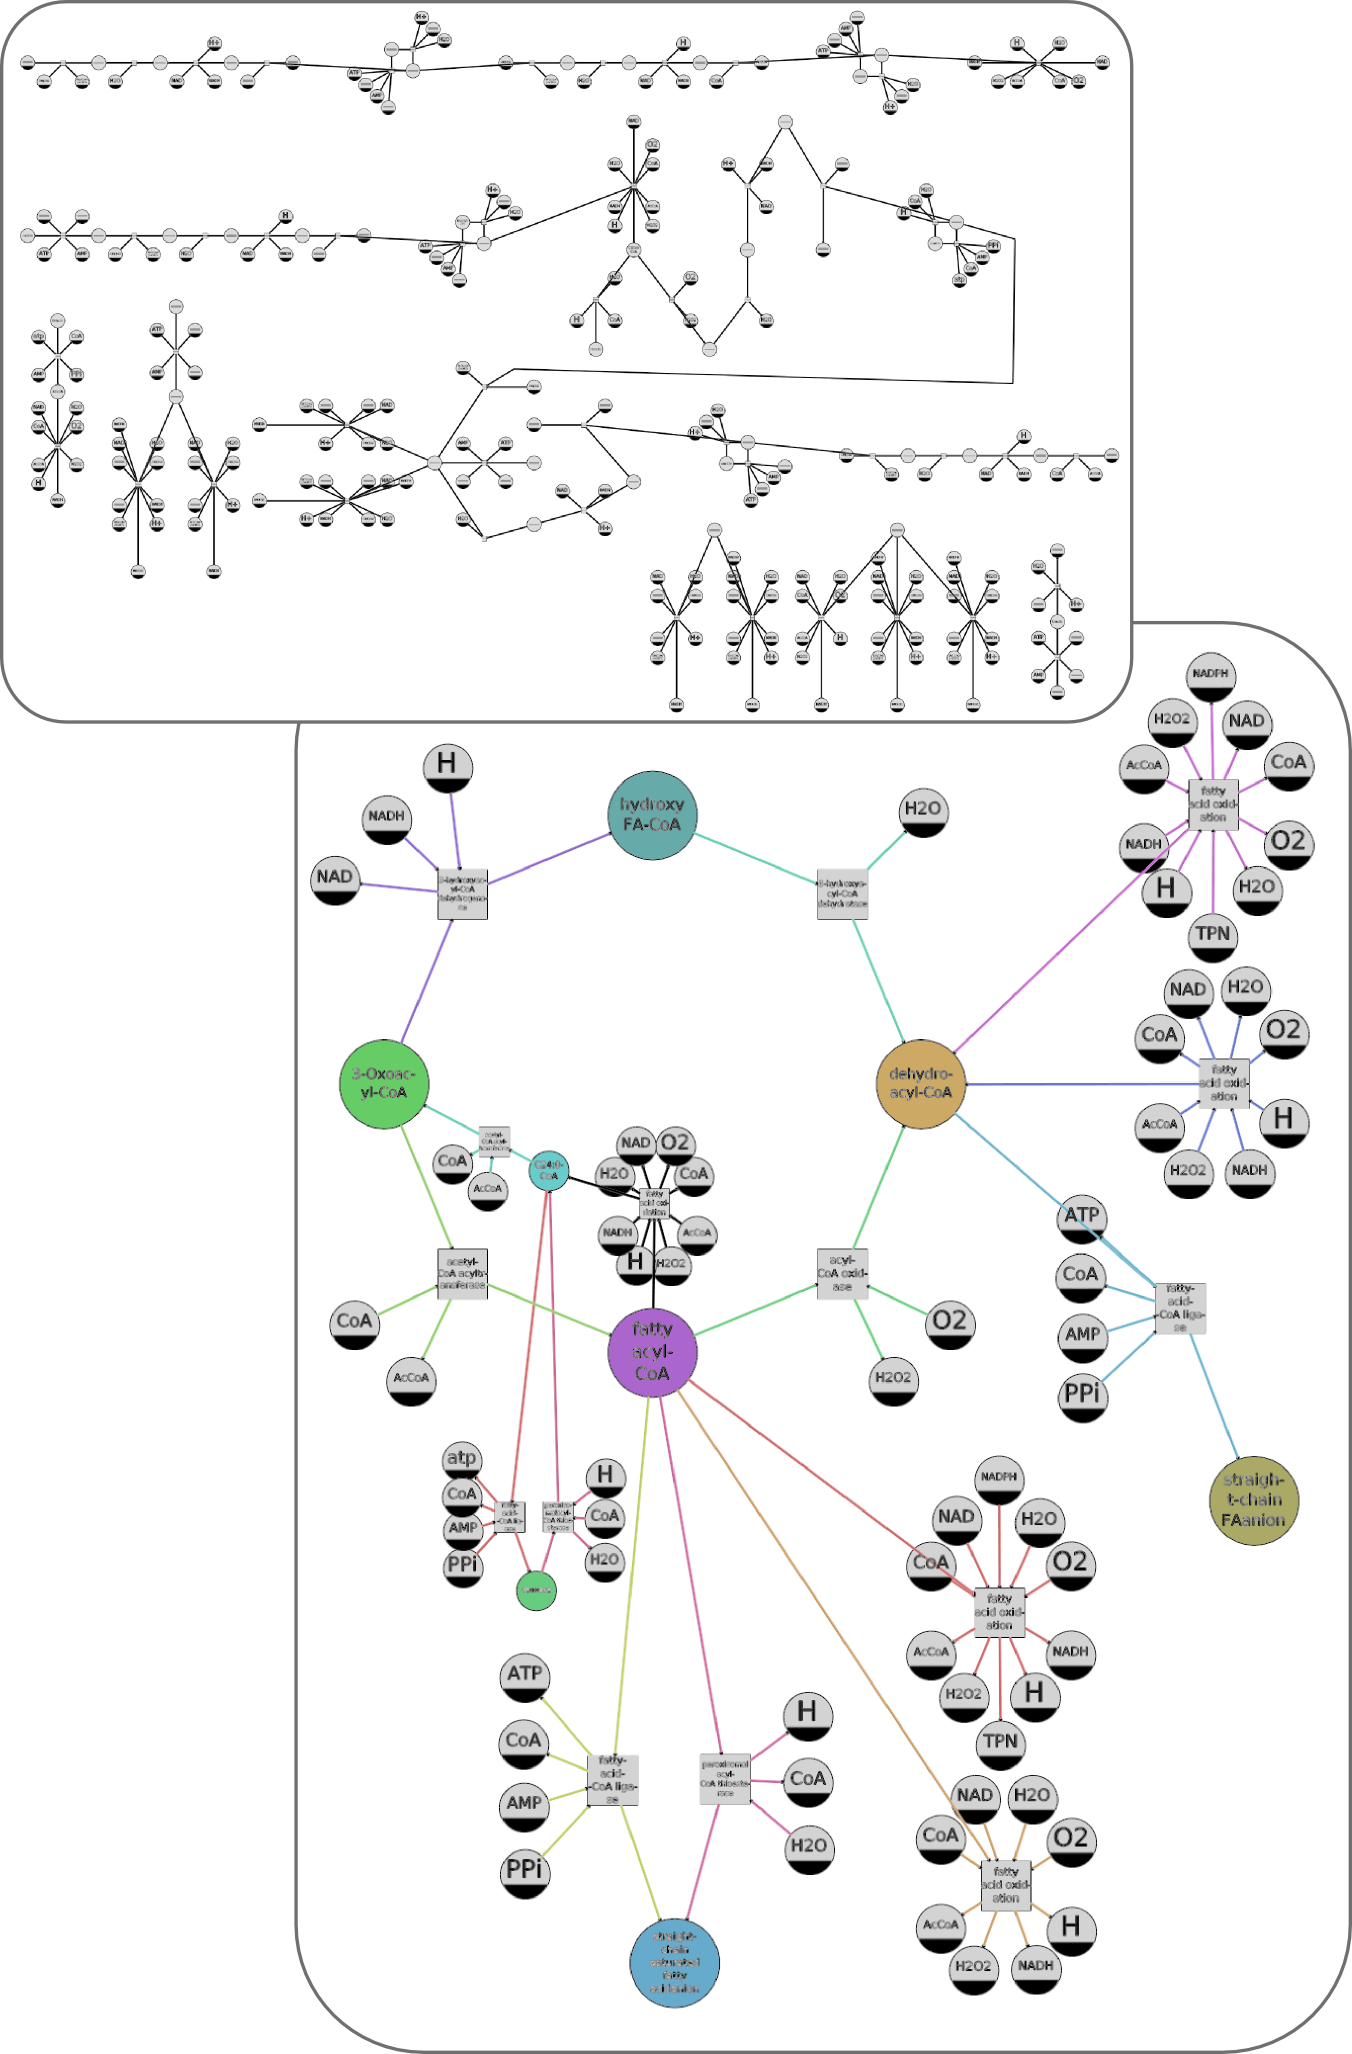
\includegraphics[scale=1]{pics/yali.png} 

      The figure shows the \textit{Yarrowia lypolitica} fatty acid oxidation model before (top right) and after (bottom left) generalization. 
      
      The generalized model describes the \textit{$\beta$-oxidation} cycle in a more generic way: as a transformation of \textit{fatty acyl-CoA} into \textit{dehydroacyl-CoA}, then into \textit{hydroxyacy fatty acyl-CoA}, \textit{3-ketoacyl-CoA}, and back to \textit{fatty acyl-CoA} (with a shorter carbon chain); while the specific model describes the same process in more details, specifying those reactions for each of the \textit{fatty acyl-CoA} species presented in the organisms' cell (e.g. \textit{decanoyl-CoA}, \textit{dodecanoyl-CoA}, etc.). The latter, more precise model, is needed for simulation, while the more general one is clearer to a human, and reveals the main properties of the model. For example, the generalized model highlights the fact that there is a particularity concerning \textit{stearoyl-CoA}: there exists a "short-cut" reaction, producing it directly from another \textit{fatty acyl-CoA}, avoiding the usual four-reaction beta-oxidation chain, used for other \textit{fatty acyls-CoA}.
      
      (The figure is produced using the Tulip~\cite{Auber04} graph visualization tool.)
\caption{Generalization of the \textit{Yarrowia lypolitica} model}
\label{fig:yali}
\end{figure}

\begin{figure}
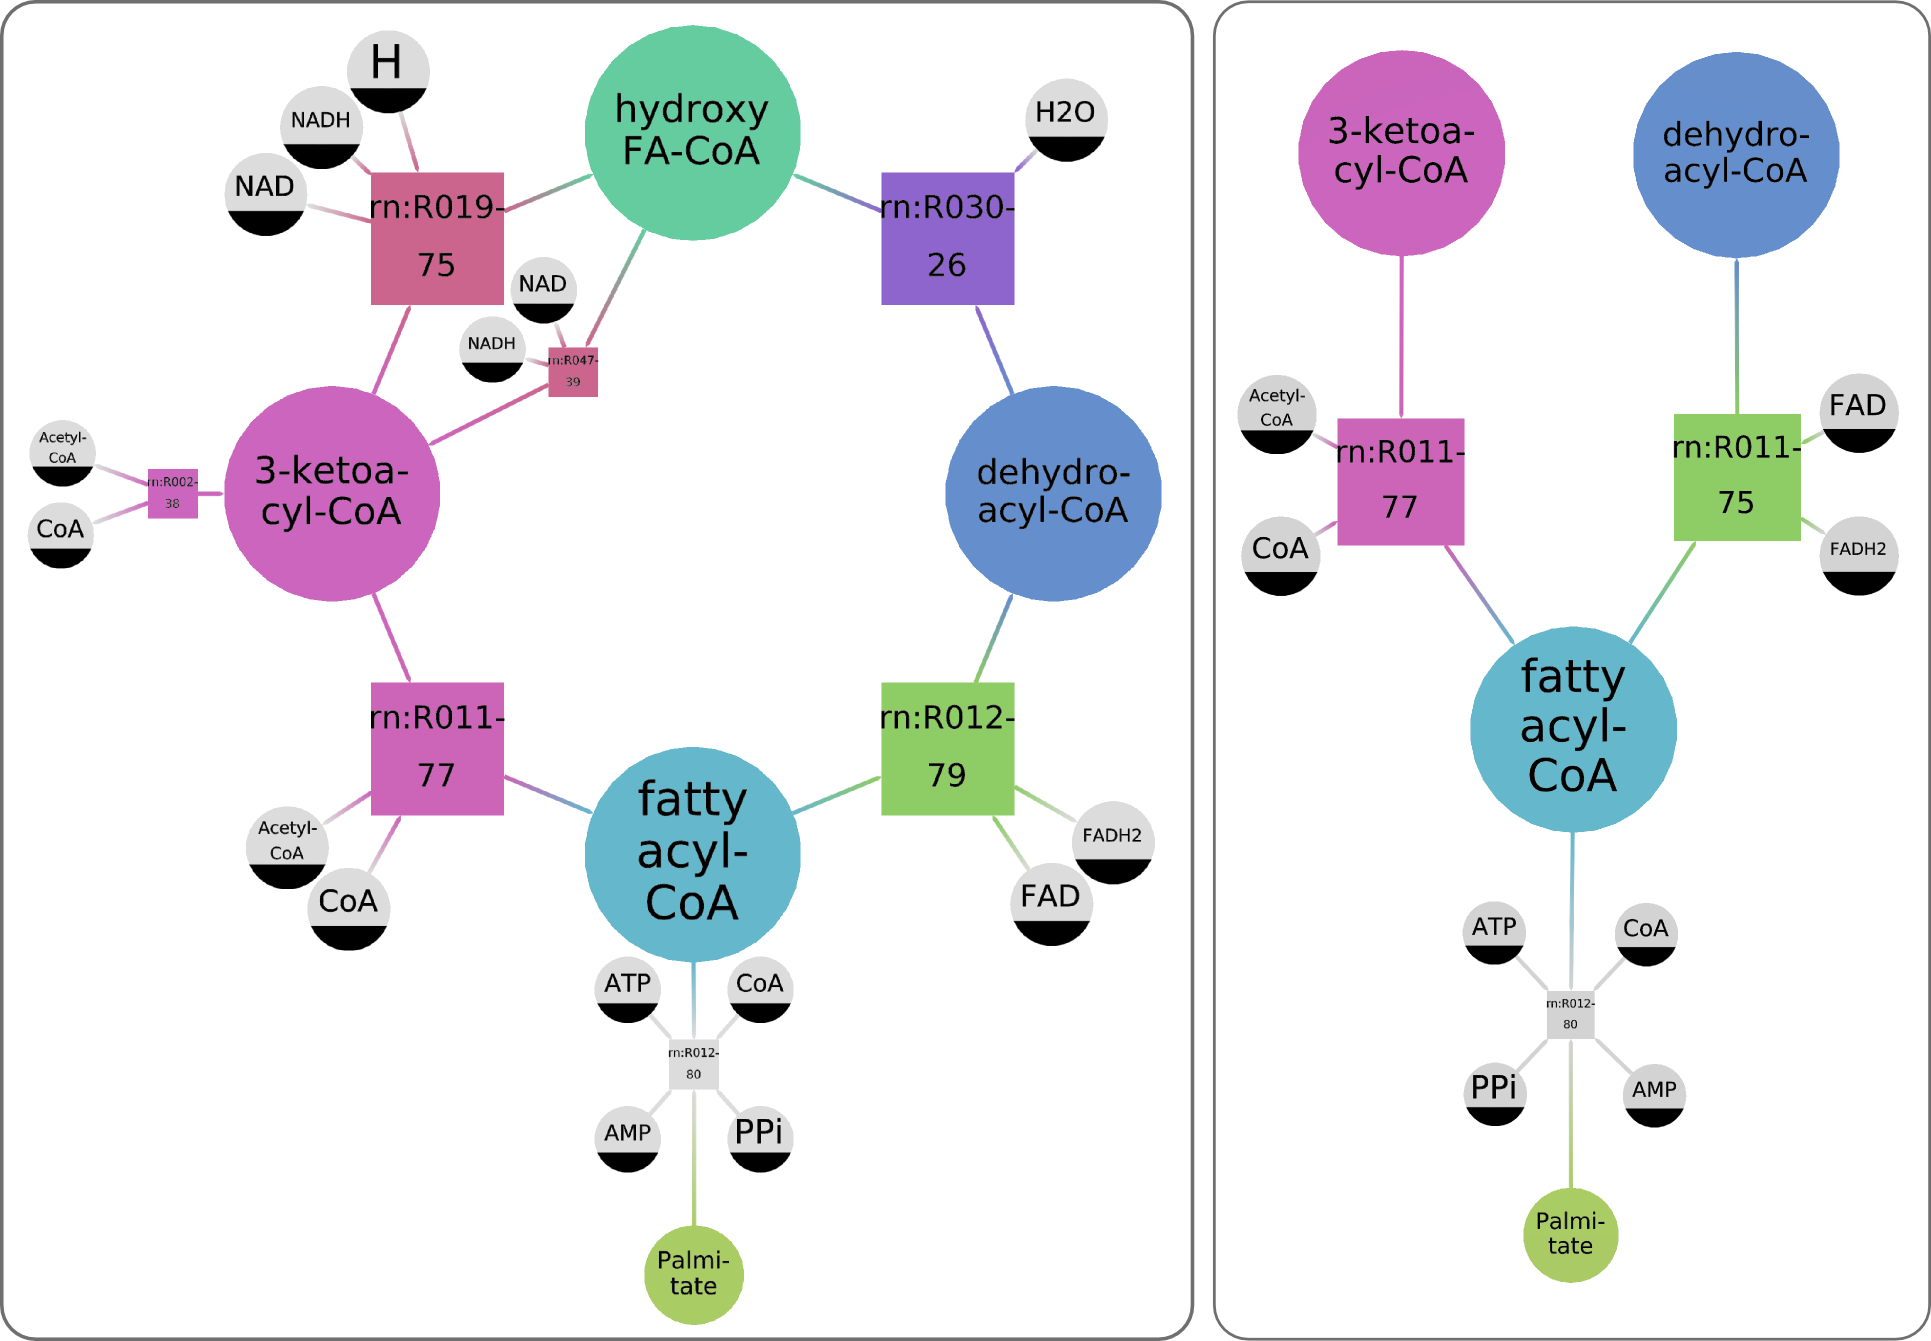
\includegraphics[]{pics/sace_ecoli.png} 

      The figure shows the generalizations of \textit{Escherichia coli} (left) and \textit{Saccharomyces cerevisiae} (right) fatty acid oxidation models.
      
      Generalization makes mistakes in the initial model more prominent. For example, in the generalized model of \textit{Saccharomyces cerevisiae} fatty oxidation is not a cycle, as it is in the generalized model of \textit{Escherichia coli}.  This is caused by the missing reactions operating with \textit{hydroxy fatty acyls-CoA}, present in the \textit{Escherichia coli} model.
      
      (The figure is produced using the Tulip graph visualization tool.)
\caption{Generalization of the \textit{Escherichia coli} and \textit{Saccharomyces cerevisiae} models}
\label{fig:gen}
\end{figure}


\section*{Conclusion}
TODO: We can merge, compare, etc. models using this technique.

\newpage
%	\section*{Discussion}
%		Generalization as rules: given an ontology and a population of models, 
%we can define a most informative set of graph rewriting rules
%
%Simplified model is easier to visualize.
%
%		Possible to the community to impose levels of abstraction: ChEBI slims as GO slims
%		
%		"isa" reaction - another approach
%			
%







%%%%%%%%%%%%%%%%%%%%%%%%%%%%%%%%%%%%%%%%%%%%%%%%%%%%%%%%%%%%%
%%                  The Bibliography                       %%
%%                                                         %%              
%%  Bmc_article.bst  will be used to                       %%
%%  create a .BBL file for submission, which includes      %%
%%  XML structured for BMC.                                %%
%%  After submission of the .TEX file,                     %%
%%  you will be prompted to submit your .BBL file.         %%
%%                                                         %%
%%                                                         %%
%%  Note that the displayed Bibliography will not          %% 
%%  necessarily be rendered by Latex exactly as specified  %%
%%  in the online Instructions for Authors.                %% 
%%                                                         %%
%%%%%%%%%%%%%%%%%%%%%%%%%%%%%%%%%%%%%%%%%%%%%%%%%%%%%%%%%%%%%

\newpage
{\ifthenelse{\boolean{publ}}{\footnotesize}{\small}
 \bibliographystyle{bmc_article}  % Style BST file
  \bibliography{db}
 }     % Bibliography file (usually '*.bib' ) 

%%%%%%%%%%%

\ifthenelse{\boolean{publ}}{\end{multicols}}{}


\end{bmcformat}
\end{document}







